\documentclass[12pt]{article}
\usepackage[utf8]{inputenc}

\usepackage{tabularx}
\usepackage{multirow}
\usepackage{graphicx}

% \title{AI-project-2019}
% \author{thanhhungqb }
% \date{May 2019}

\usepackage[legalpaper, margin=1in]{geometry} % landscape
\begin{document}

% \maketitle

\begin{table}[]
% \begin{tabularx}{\textwidth}{X}
\begin{tabular}{|l|l|l|l|l|l|}
\hline
\begin{tabular}[c]{@{}l@{}}Project\\ Title\end{tabular} & \multicolumn{3}{c|}{\textbf{\begin{tabular}[c]{@{}l@{}}Facial emotion recognition\\ with latent topics modeling\\ on local features\end{tabular}}} & Date & 2019.05.27 \\ \hline
Name & \hspace{.5cm} Vo Thanh Hung \hspace{.5cm} & Student ID & \hspace{0.5cm} 198554 \hspace{0.5cm} & Evaluation &  \\ \hline
\end{tabular}
\end{table}
% \end{tabularx}


\section{Project Overview}
% In this section
% - Why do you do this project?
% - Why is this project important?
% Etc., describe the background, necessity and importance of the project.

In this study, I am going to discover re-presentation of image features and apply to facial emotion recognition (FER) problem.
There are many feature extraction method including Scale Invariant Feature Transform \cite{Lowe2004} (SIFT), Speeded Up Robust Features \cite{Bay06} (SURF), KAZE features \cite{alcantarilla2012kaze}, etc.
In this project, SIFT, SURF and KAZE are used.
Each of above method will generate a set of vector from given image.
To use extracted features to most of recognition problem, we have to re-presentation them.
Bag-of-Features \cite{nowak2006sampling} was wide used for this step which the idea transform from Bag-of-Words in natural language processing (NLP).
In this study, I address not only one kind of feature, but also multi-features kind, meaning from some difference feature extraction method.
So, I hope that the result can be improve and general compared to single method.

I am going to apply for FER problem and on some special popular dataset.
The problem is expected that combine many type of local features can present and easy understand emotion in image.
% There are another assumption, that facial features are not change too much and prevent with many [TO-DO pose]...

After that, some popular traditional machine learning methods are used to facial emotion recognition including Support Vector Machine \cite{suykens1999least} (SVM), Random Forest \cite{liaw2002classification}.

\section{Key technology}
% - Describe some of the key skills required to carry out the project.
% - Summarize the necessary related knowledge about artificial intelligence technology used for the project..
Many related technologies are show as below.

% [TO-DO feature]

Feature extraction:
\begin{itemize}
    \item Scale Invariant Feature Transform \cite{Lowe2004} (SIFT)
    \item Speeded Up Robust Features \cite{Bay06} (SURF)
    \item KAZE features \cite{alcantarilla2012kaze}
    % \item \cite{Pang2012} 
    % \item \cite{Sun:2016:EMV:2988257.2988270}
\end{itemize}

% [TO-DO feature normalization]

% [TO-DO LDA, HDP]
Topics modeling:
\begin{itemize}
    \item Latent Dirichlet Allocation \cite{blei2003latent, Blei2003} (LDA)
    \item Hierarchical Dirichlet Process \cite{teh2005sharing} (HDP)
\end{itemize}

% [TO-DO machine learning]
Machine learning classifier:
\begin{itemize}
    \item Support Vector Machine \cite{suykens1999least} (SVM)
    \item Random Forest \cite{liaw2002classification}
\end{itemize}

% [TO-DO? transfer model]

\section{Project contents} \label{sec:project-contents}
% In this section, you will write something about the actual
% - Structure of system
% - Basic algorithm
% - Specific implementation details, etc.


% [TO-DO add system architect]
Figure \ref{fig:system-architect} show overall system architect.
The input image goes through feature extractor block to get all features.
These block including SIFT, SURF and KAZE.
Then Bag-of-Features does clustering and make fixed vocabulary.
From here, there are two branches to implement two difference approaches.
First approach is to directly use Bag-of-Features and classifier.
The other approach is to modeling features use HDP and then represent image before goes through classifier block as previous.
Two approaches work independence to compare.
\begin{figure}[h!]
    \centering
    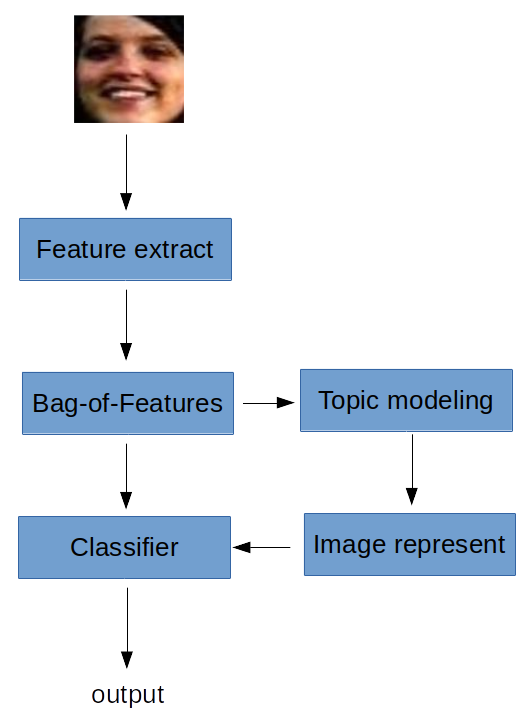
\includegraphics[width=0.45\textwidth]{system-arch-cropped.png}
    \caption{Facial emotion recognition system architect} \label{fig:system-architect}
\end{figure}

Below subsections show description for each block.

% ----------------------------
% feature extraction
% ----------------------------
\subsection{Features extraction}
This step aims to extract features from images.
The OpenCV toolbox \cite{opencv_library} was used to perform this task.
The input is an image, the output is features.
The feature size of SIFT, SURF and KAZE are 128, 64  and 64, in this order.

After extracted, all features vector are normalize use l2 normalization.

% ----------------------------
% Bag-of-Feature
% ----------------------------
\subsection{Bag-of-Features}
In our case, there are many kind of feature vectors from difference extractor, that mean they have difference size of vector.
The SIFT feature size is 128 while SURF feature size is 64 and similar for KAZE.
Bag-of-Features technique are wide used to represent image features.
From normalized features, the clustering is used to make the number of cluster $K$ based on distance of features.
The K-means clustering algorithm \cite{hartigan1979algorithm} was widely used, and Euclidean distance also used here.
$K$, the number of cluster is number of vocabulary.
All feature belong to one cluster is same \textit{word} which centroid of cluster is represent for them.

Then the image is represent as a vector length $K$, each value in the vector is for one word.
Word order is not considered here.
Term Frequency (TF) for each word is calculated and make vector.
In this case, I am going to use both TF and IDF (Inverse Document Frequency) to make vector and compare result.
Both TF and IDF concepts are come from NLP.


% ----------------------------
% build hdp model for feature
% ----------------------------
\subsection{Features modeling}
This part of study tries to modeling features of image in an another way than Bag-of-Features.
In this project, latent topics modeling are explore, one another techniques from NLP.
The main idea is to discover the related of hidden topics from words, features.

Latent Dirichlet Allocation \cite{blei2003latent, Blei2003} is probabilistic for describing whether a subject are present in each document relative to a given article topic model.
There the number of topics is set and the probabilities of words belongs to each topic and the probabilities of documents belongs to each topic are estimate.
In our case, the words are represent vectors and images are documents.

Hierarchical Dirichlet Process \cite{teh2005sharing} (HDP) is a improvement version of LDA where number of topic need not given, they will be estimate too.

There are some use case and modified version of LDA and HDP were studied by Hu et al. in \cite{Hu2009} and Cao et al. in \cite{Cao2007}.

In this project, I am going to modeling features by latent topic and HDP is used.

% ----------------------------
% classifier
% ----------------------------
% SVM
% Random forest
% NB
% KNN?
\section{Classifier}
In this study, we use some popular traditional machine learning to classify including SVM \cite{suykens1999least}, Random forest \cite{liaw2002classification}, Naive Bayes.


\section{Schedule}
- Record the work schedule for section \ref{sec:project-contents} by dividing the project contents for a week.

\begin{table}[h!]
\begin{tabular}{|c|c|c|c|c|}
\hline
\multirow{2}{*}{Work Contents} & \multicolumn{3}{c|}{Schedule} & Remarks \\ \cline{2-5} 
 & May $20^{th}$ & May $27^{th}$ & June $3^{rd}$ &    \\ \hline
Internet search and paper collection & \textless--- ---\textgreater &  &  &      \\ \hline
Paper reading & \textless---  & ---\textgreater &  &      \\ \hline
Data Analysis &  & \textless--- & ---\textgreater &    \\ \hline
\end{tabular}
\end{table}

\section{Others}

\bibliographystyle{ieeetr}
\bibliography{library,library-tools,a} 

\end{document}
